\documentclass[12pt]{article}
\usepackage[utf8]{inputenc}
\usepackage[spanish]{babel}
\decimalpoint
\usepackage{amsmath}
\usepackage{amsthm}
\usepackage{amssymb}
\usepackage{graphicx}
\usepackage[margin=0.9in]{geometry}
\usepackage{fancyhdr}
\usepackage[inline]{enumitem}
\usepackage{float}
\usepackage{cancel}
\usepackage{bigints}
\usepackage{color}
\usepackage{xcolor}
\usepackage{listings}
\usepackage{listingsutf8}
\usepackage{algorithm}
\usepackage{tocloft}
\usepackage[none]{hyphenat}
\usepackage{graphicx}
\usepackage{grffile}
\usepackage{tabularx}
\usepackage[nottoc,notlot,notlof]{tocbibind}
\renewcommand{\cftsecleader}{\cftdotfill{\cftdotsep}}
\pagestyle{fancy}
\setlength{\headheight}{15pt} 
\lhead{Introducción a los sistemas operativos}
\rhead{\thepage}
\lfoot{Sistemas Operativos}
\renewcommand{\footrulewidth}{0.5pt}
\setlength{\parskip}{0.5em}
\newcommand{\ve}[1]{\overrightarrow{#1}}
\newcommand{\abs}[1]{\left\lvert #1 \right\lvert}

\definecolor{pblue}{rgb}{0.13,0.13,1}
\definecolor{pgreen}{rgb}{0,0.5,0}
\definecolor{pred}{rgb}{0.9,0,0}
\definecolor{pgrey}{rgb}{0.46,0.45,0.48}
\lstset{tabsize=1}

\newcommand{\tabitem}{~~\llap{\textbullet}~~}
\newcommand{\subtabitem}{~~~~\llap{\textbullet}~~}

\bibliographystyle{IEEEtran}
\usepackage{listings}
\lstdefinestyle{customc}{
  belowcaptionskip=1\baselineskip,
  breaklines=true,
  frame=L,
  xleftmargin=\parindent,
  language=C,
  showstringspaces=false,
  basicstyle=\footnotesize\ttfamily,
  keywordstyle=\bfseries\color{green!40!black},
  commentstyle=\itshape\color{purple!40!black},
  identifierstyle=\color{blue},
  stringstyle=\color{orange},
}

\lstdefinestyle{customasm}{
  belowcaptionskip=1\baselineskip,
  frame=L,
  xleftmargin=\parindent,
  language=[x86masm]Assembler,
  basicstyle=\footnotesize\ttfamily,
  commentstyle=\itshape\color{purple!40!black},
}

\lstset{escapechar=@,style=customc}
\begin{document}
		\begin{titlepage}
			\begin{center}
				
				% Upper part of the page. The '~' is needed because \\
				% only works if a paragraph has started.
				
				\noindent
				\begin{minipage}{0.5\textwidth}
					\begin{flushleft} \large
						
\includegraphics[width=0.3\textwidth]{ipn.png}
					\end{flushleft}
				\end{minipage}%
				\begin{minipage}{0.55\textwidth}
					\begin{flushright} \large
						
\includegraphics[width=0.7\textwidth]{escom.png}
					\end{flushright}
				\end{minipage}
				
				\textsc{\LARGE Instituto Politécnico Nacional}\\[0.5cm]
				
				\textsc{\Large Escuela Superior de Cómputo}\\[1cm]
				
				% Title
				
				{ \huge Práctica No.1 \\[1cm] }
				{\huge Introducción a los sistemas operativos\\[1cm]}
				
				{ \Large Unidad de aprendizaje: Sistemas Operativos} \\[1cm]
				
				{ \Large Grupo: 3CM4 } \\[1cm]
				
				\noindent
				\begin{minipage}{0.5\textwidth}
					\begin{flushleft} \large
						\emph{Integrantes del equipo:}\\
						
						\begin{tabular}{ll}
					     Domínguez Morán Joaquín\\
					     Carrillo Balcazar Eduardo Yair\\
					     Ruiz López Luis Carlos\\
					\end{tabular}
					\end{flushleft}
				\end{minipage}%
				\begin{minipage}{0.5\textwidth}
					\begin{flushright} \large
						\emph{Profesor:} \\
						Jorge Cortes Galicia 
					\end{flushright}
				\end{minipage}
				
				\vfill
				
				% Bottom of the page
				{\large 3 de septiembre de 2018}
			\end{center}
		\end{titlepage}
	
	\tableofcontents
    \newpage
    
\section{Competencias.}
El alumno analiza el sistema operativo Linux y Windows mediante el uso de su interfaz de comandos respectiva para comparar sus características principales y diferenciarlos en su ambiente de trabajo.

El alumno desarrolla aplicaciones en lenguaje C para los sistemas operativos Linux y Windows.

\section{Desarrollo.}
\subsection{ Sistema Operativo Linux}
Linux, es un sistema operativo libre tipo Unix; multiplataforma, multiusuario y multitarea. 
\subsubsection{Distribuciones de Linux.}
Linux se le encuentra normalmente en forma de compendios conocidos como distribuciones o distros, a las cuales se les han adicionado selecciones de aplicaciones y programas para descargar e instalar las mismas. El propósito de una distribución es ofrecer Linux como un producto final que el usuario pueda instalar, cumpliendo con las necesidades de un grupo de usuarios o bien del público general.

Las principales distribuciones de Linux son: 
\begin{itemize}
    \item {Ubuntu: La distribución más grande y utilizada del mundo, desarrollada y mantenida por la empresa Canonical, se orienta a usos generales y se caracteriza por su compatibilidad de software y facilidad de uso equiparable a Mac OS X o Windows, es la más representativa del sistema operativo Linux.}
    \item {Fedora: Distribución para propósitos generales, que se caracteriza por ser estable y seguro, la cual es desarrollada y mantenida por la empresa Red Hat y una comunidad internacional de ingenieros, diseñadores gráficos y usuarios que informan de fallos y prueban nuevas tecnologías. Sus usos se orientan más al desarrollo de software y servidores.}
    \item{ Debian: Uno de sus principales objetivos es separar en sus versiones el software libre del software no libre. El modelo de desarrollo es independiente a empresas, creado por los propios usuarios, sin depender de ninguna manera de necesidades comerciales. Debian no vende directamente su software, lo pone a disposición de cualquiera en Internet, aunque sí permite a personas o empresas distribuir comercialmente este software mientras se respete su licencia.}
\end{itemize}
\newpage
\subsubsection{Distribución Debian.}
Se ha deicido utilizar Debian debido a que ofrece: 
\begin{itemize}
    \item {La disponibilidad en varias arquitecturas. La versión estable incluye soporte para 12 plataformas.}
    \item {Una amplia colección de software disponible}
    \item{Un grupo de herramientas para facilitar el proceso de instalación y actualización del software.}
    \item{Su compromiso con los principios y valores involucrados en el movimiento del Software Libre.}
    \item{No tiene marcado ningún entorno gráfico en especial, pudiéndose no instalar ninguno.}
\end{itemize}

\subsubsection{Funcionalidades.}
Una funcionalidad de Linux que no se encuentran en Windows son la habilidad de descargar programas desde la terminal de una manera fácil, escribiendo un “sudo apt-get” y tecleando el programa a descargar, se pueden adquirir ciertos programas, lo cual no existe integrado en Windows. Desde un punto de vista sin experiencia, esto podría ser una desventaja, ya que en Windows se instalan programas desde la página de descargas del programa y se corre un wizard para llevar a cabo la instalación personalizada del producto. 

A grandes rasgos Linux se basa en los comandos que puede llevar a cabo su terminal, y de vez en cuando en programas accedidos fuera de ella, mientras que en Windows, la terminal es, en ciertas ocaciones, lo último que se utiliza para correr un programa o compilarlo, dado que existen IDEs que facilitan esto.


\newpage
\subsubsection{Comandos.}
A continuación se describen los usos de los comandos principales del sistema opertivo Linux.

    \\
 
    \begin{tabular}{
			|p{5cm}|p{9cm}||}
		
			\hline
			\textbf{ Comando} & \textbf{  Función}\\ 
			\hline
			\hline ls & Enumerar los contenidos del directorio.\\
			\hline chmodG& Cambiar bits a modo de archivo.\\
			\hline vi & Puede ser usado para editar todo tipo de texto sin formato. Es especialmente útil para editar programas.\\
			\hline pwd & Imprimir el nombre del directorio actual o de trabajo.\\
			\hline clear & Limpiar la pantalla de la terminal. \\
			\hline  cd & Nos permite acceder a una carpeta o directorio de Linux.\\
			\hline cat & Concatenar archivos e impimir la salida estandar.\\
			\hline grep & Imprimir lineas que coincidan con un patrón.\\
			\hline rm & Eliminar archivos o directorios.\\
			\hline ps & Informar de los procesos que se están ejecutando actualmente.\\
			\hline cp & Copiar archivos y directorios.\\
			\hline mv & Renombrar archivos.\\
			\hline mkdir & Crear directorios.\\
			\hline rmdir & Eliminar directorios vacios.\\
			\hline whoami & Imprimir el nombre de usuario asociado con la identificación del usuario efectivo actual.\\
			\hline
			\end{tabular}\
\newpage
\paragraph{ Ejecución de comandos: }
\begin{itemize}
    \item Comandos ls y ls-l:
    
    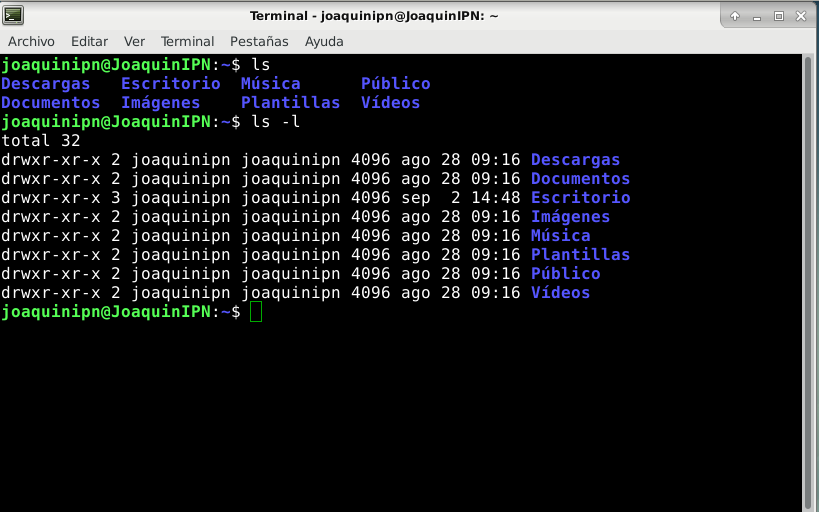
\includegraphics[scale=.5]{1.png}
    
    \item Comando ls-a:
    
    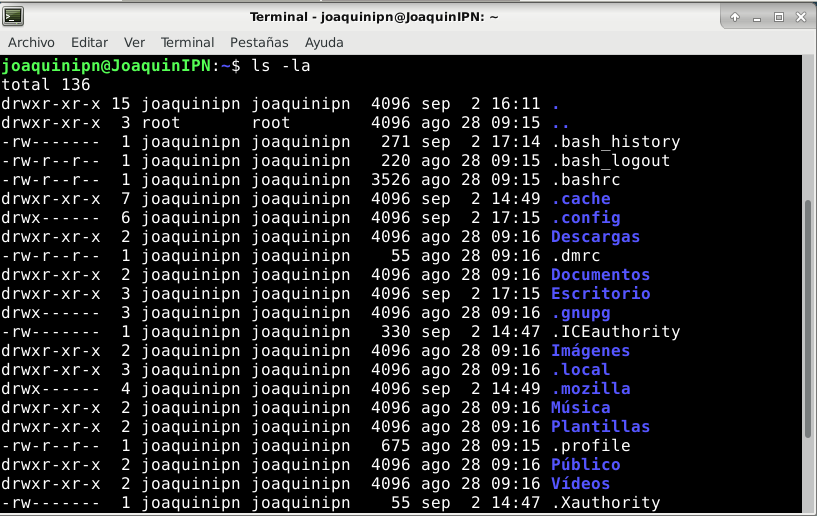
\includegraphics[scale=.5]{2.png}
    
    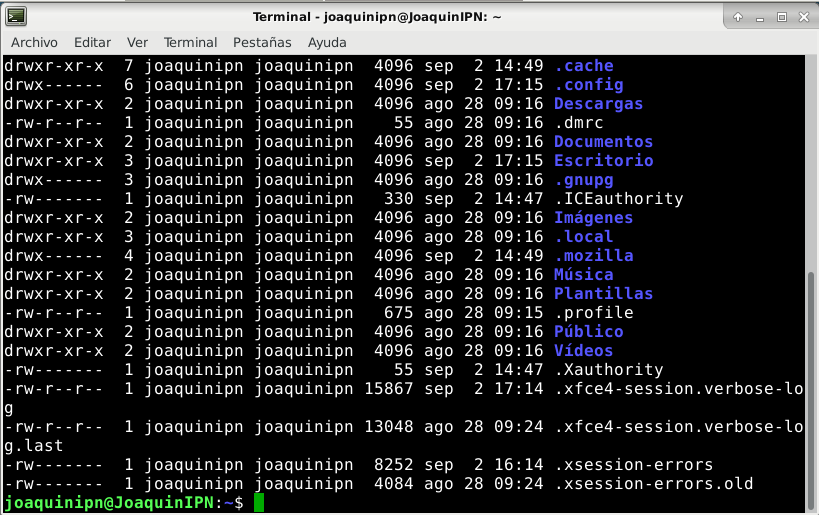
\includegraphics[scale=.5]{3.png}
    
    \item Comando  pwd :
    
    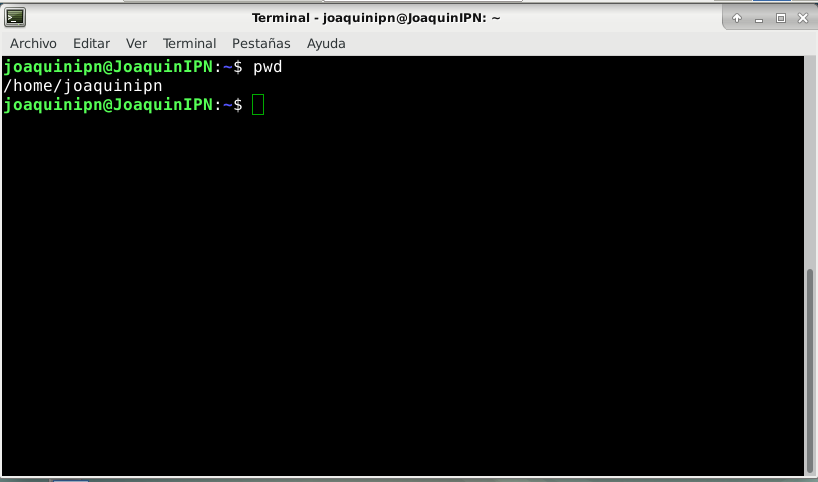
\includegraphics[scale=.5]{4.png}
    \newpage
    \item Comando clear :
    
    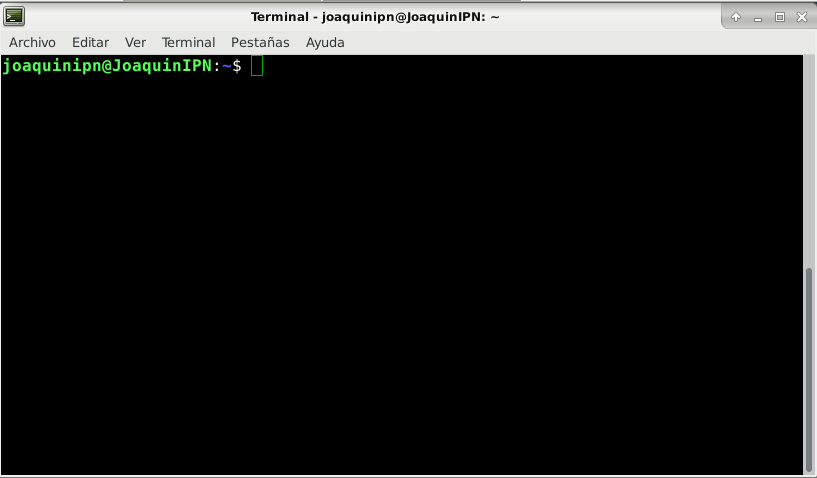
\includegraphics[scale=.5]{5.png}
    
    \item Comandos cd , cat, ls -la more , rm , ps  :
    
    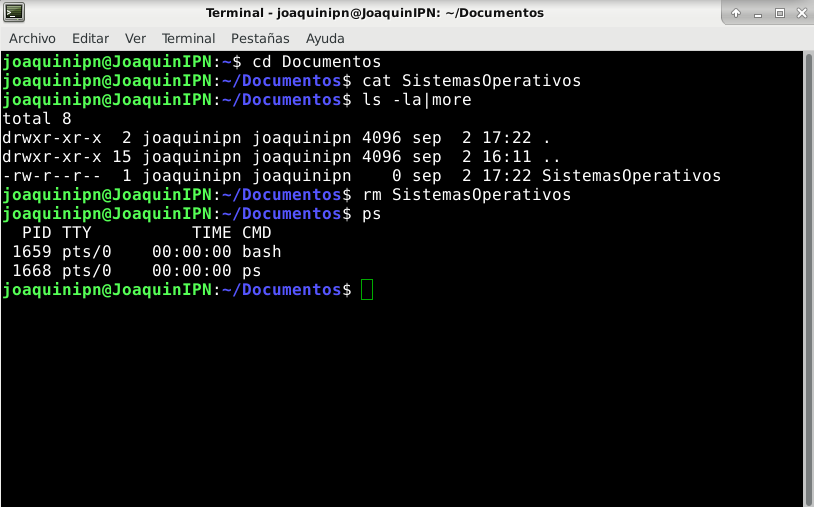
\includegraphics[scale=.5]{6.png}
    
    \newpage
    
    \item Comando cp:
    
    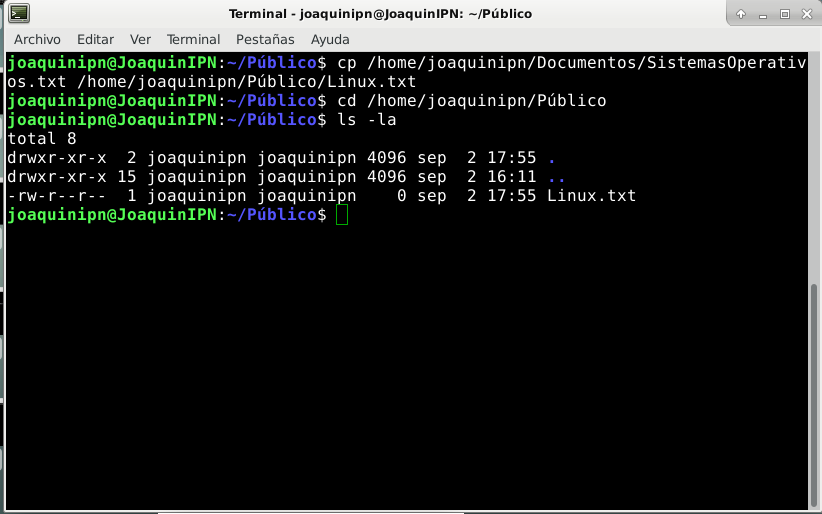
\includegraphics[scale=.5]{8.png}

    \item Comando  mv :
    
    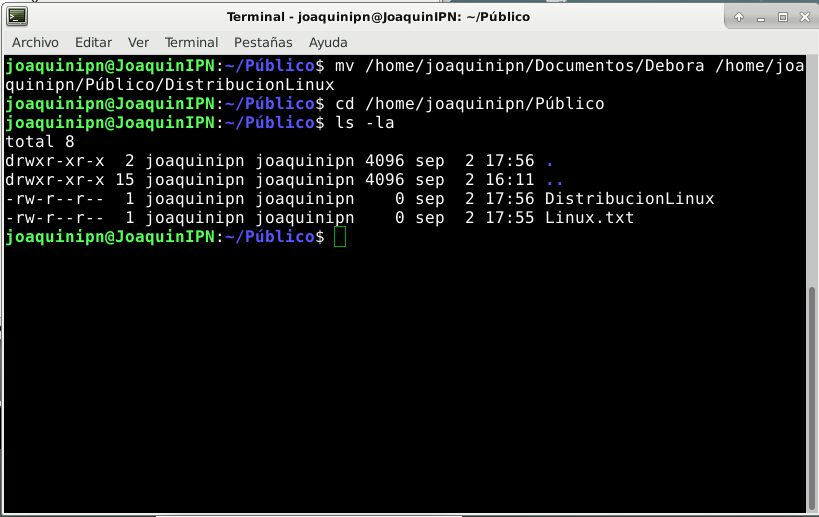
\includegraphics[scale=.5]{9.png}
    
    \newpage
 
    \item Comandos mkdir, rmdir y whoami :
    
    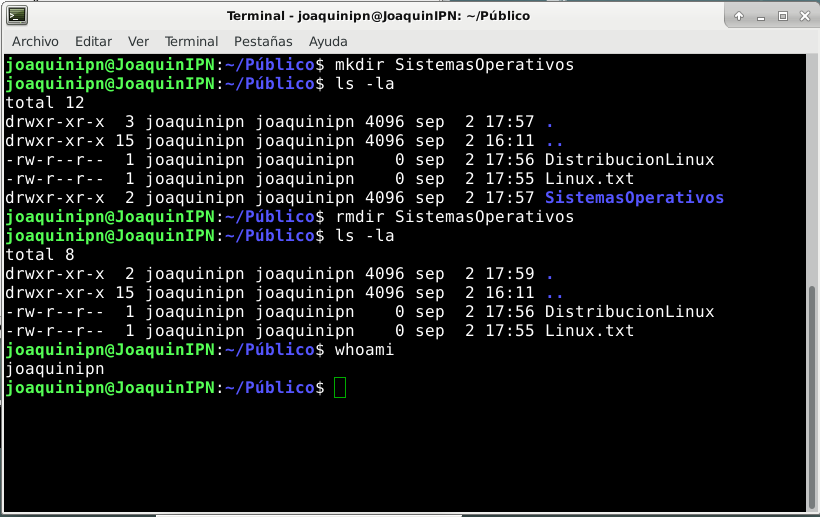
\includegraphics[scale=.5]{10.png}

\paragraph{ Diversas opciones que se utilizan los diferentes comandos : }

    \item ls:
    \begin{itemize}
        \item -a : No ignorar entradas que comienzan con .
        \item -A: No enumerar implícitamente y con -l , imprimir el autor de cada archivo.
        \item -l: Imprimir el autor de cada archivo.
        \item -1: Enumerar un archivo por línea.
        \item - X: Ordenar alfabéticamente por extensión de entrada.
        \item -w: Asumir ancho de la pantalla en lugar del valor actua.
        \item -U: No ordenar; entradas de la lista en orden de directorio.
        \item  -u: Con -lt : ordenar por, y mostrar, el tiempo de acceso con -l : tiempo de acceso al espectáculo y ordenar por nombre de otro modo: ordenar por tiempo de acceso.
        \item -t: Ordenar por fecha de modificación.
        \item -S: Ordenar por tamaño de archivo.
        \item -s: Imprimir el tamaño asignado de cada archivo, en bloques.
        \item -R: Lista subdirectorios recursivamente.
        \item -r: Orden inverso al ordenar.
        \item -Q: Encerrar los nombres de entradas en comillas dobles.
        \item -q: Impresión  en lugar de los caracteres no gráficos.
        \item -p : Indicador de directorios.
        \item -N: Imprimir los nombres de entradas primas.
        \item - m: Llenar ancho con una lista separada por comas de entradas
        \item -l: Utilizar un formato larga lista
        \item -i: Imprimir el número de índice de cada archivo
        
    \end{itemize}
    
    \item pwd :
    
    \begin{itemize}
        \item -L: Usa todos los PWD, incluso si contiene enlaces simbólicos.
        \item -P: Evitar todos los enlaces simbólicos.
    \end{itemize}
    
    
    
    \item cd: 
        \begin{itemize}
        \item -a: Modo de control de acceso.
        \item -m: Modo de lectura.
        \item -d: Establecer la depuración. 
        \item -x: Estabcer la salida en un valor hexadecima.
        \item -j: No mostrar caracteres de valor hexadecimal.
        \item -n: Establecer el número de sectores a leer.
        \item -V: Muestra la versión e información de derechos de autor y salida.
    \end{itemize}
    
    \item cat
    \begin{itemize}
        \item -b: Número de lineas de salida vacias.
        \item -n: Numerar todas las líneas de salida
        \item -s: Suprimir las líneas de salida vacías repetidas.
    \end{itemize}
    
    \item rm 
    \begin{itemize}
        \item -f: Ignorar los archivos no existentes, no pronta.
        \item -i: Preguntar antes de cada extracción.
        \item -I: Preguntar una vez antes de sacar más de tres archivos, o al retirar de forma recursiva.
        \item -r, -R :Eliminar directorios y sus contenidos de forma recursiva.
        \item -v: Explicar lo que se está haciendo.
    \end{itemize}
    \item ps 
    \begin{itemize}
        \item -A: Seleccionar todos los procesos.
        \item -N: Seleccionar todos los procesos excepto aquellos que cumplen las condiciones especificadas.
        \item -T: Seleccionar todos los procesos asociados a una terminal.
        \item -a:Seleccionar todos los procesos excepto los dos líderes de sesiones  y procesos que no están asociados con una terminal.
        \item -re:Seleccionar todos los procesos excepto los líderes de la sesión.
        \item -e:Seleccionar todos los procesos.
        \item -r:Restringir la selección a los procesos que se ejecutan solamente.
    \end{itemize}

    \item cp:
    \begin{itemize}
        \item --backup : Hacer una copia de seguridad de cada archivo de destino existente.
        \item --copy-contents: Contenido de la copia de archivos especiales cuando es recursiva.
        \item -f:Si un archivo de destino existente no se puede abrir, retirar y vueler a intentarlo.
        \item -i:Confirmación antes de sobrescribR.
        \item -l: Gnerar rchivos de enlace en lugar de copiar.
        \item -u:Copiar sólo cuando el archivo de origen es más reciente que el archivo de destino o cuando el archivo de destino no se encuentra.
    \end{itemize}
    


    \item mv :
    \begin{itemize}
        \item -- backup: Hacer una copia de seguridad de cada archivo de destino existente.
        \item -f: No se preguntar antes de sobrescribir.
        \item -i: Confirmar antes de sobrescribir.
        \item -n: No sobrescribir un archivo existente.
        \item -t: Mover todos los argumentos de origen en el directorio.
        \item -u: Moverse sólo cuando el archivo de origen es más reciente que el archivo de destino o cuando el archivo de destino no se encuentra.

    \end{itemize}
    
    \item mkdir :
    \begin{itemize}
        \item -m: Establecer el modo de archivo.
        \item -p: Si es que existe ningún error , hacer directorios padre, según sea necesario.
        \item -v: Imprimir un mensaje para cada directorio creado.
        \item -Z: Establecer el contexto de seguridad de SELinux de cada directorio creado para CTX.
    \end{itemize}
    
    \item rmdir :
      \begin{itemize}
        \item -p: Eliminar el directorio y sus antecesores.
        \item -v: Salida de un diagnóstico para cada directorio procesado.
  
    \end{itemize}
    
\end{itemize}
    
\subsubsection{ Compilación y ejecución.}
      \begin{itemize}
                \item Hola Mundo
                
                   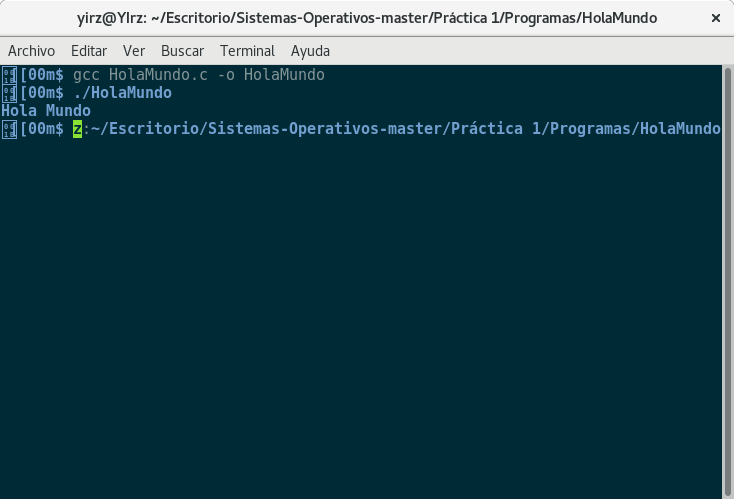
\includegraphics[scale=.5]{Imagenes/Linux/HolaMundo.png}
            
                \item Balanceo de Paréntesis
                
                  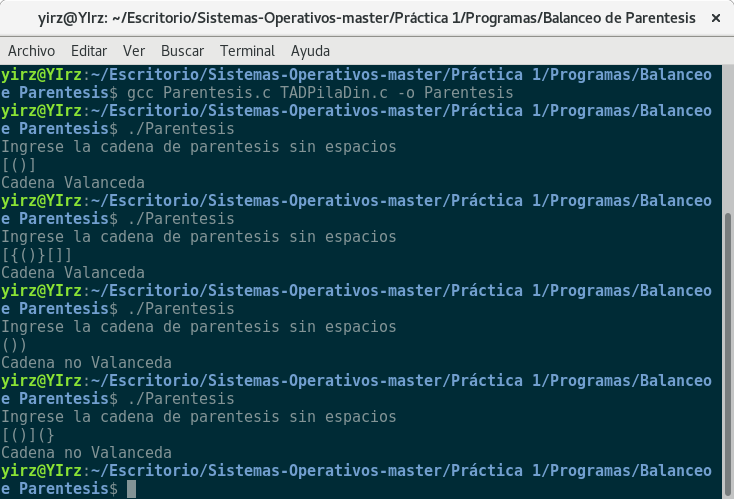
\includegraphics[scale=.6]{Imagenes/Linux/Parentesis.png}
                    
                \item Salida con astesiscos
                
                    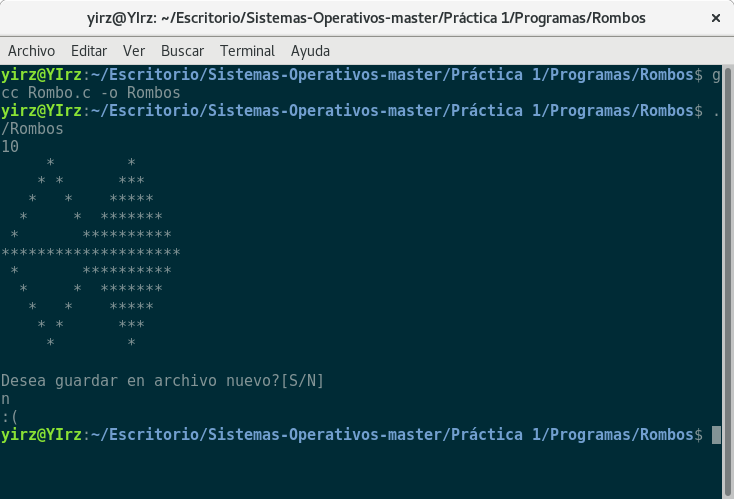
\includegraphics[scale=.6]{Imagenes/Linux/Rombo.png}
                    
                \item Torres de Hanoi\\
                    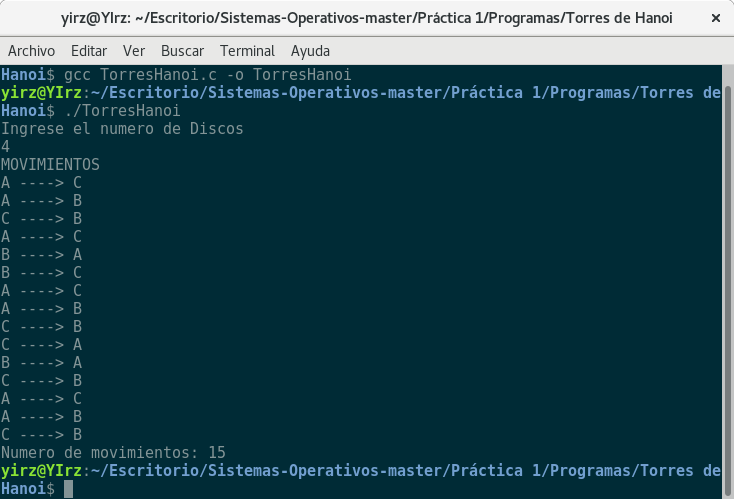
\includegraphics[scale=.6]{Imagenes/Linux/TorresHanoi.png}
                    \\
                \item Expresiones Artiméticas\\
                    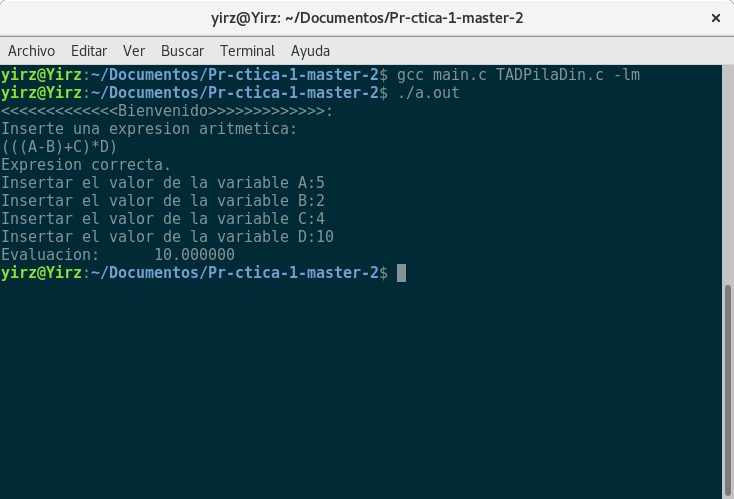
\includegraphics[scale=.6]{Imagenes/Linux/Operaciones.png}
                    
            \end{itemize}
            
\newpage
\subsection{Sistema Operativo Windows.}
\subsubsection{Comandos.}
    A continuación se describen los usos de los comandos principales del sistema opertivo Windows.
    
    \\
		\begin{tabular}{
			|p{5cm}|p{9cm}||}
			\hline
			\textbf{ Comando} & \textbf{  Función}\\ 
			\hline
			\hline DIR & Mostrar listado de archivos y directorios\\
			\hline IPCONFIG& Muestra los valores de configuración de red de TCP/IP\\
			\hline CLS & Borra la pantalla\\
			\hline VER& Muestra la versión de Microsoft Windows\\
			\hline TREE & Muestra el listado de carpetas en Windows\\
			\hline  CD & Nos permite acceder a una carpeta o directorio de Windows\\
			\hline TYPE & Muestra el contenido de uno o más archivos de texto, es decir, la extensión\\
			\hline MKDIR & Crea un directorio nuevo\\
			\hline RMDIR & Borra un directorio existente\\
			\hline DEL & Elimina uno o varios archivos\\
			\hline COPY & Copia un archivo\\
			\hline REN & Cambia el nombre de uno o más archivos\\
			\hline CHDIR & Muestra el nombre del directorio actual o cambia a otro directorio\\
			\hline ECHO & Muestra mensajes o activa y desactiva al ECO\\
			\hline FIND & Busca una cadena de texto en uno o más archivos\\
			\hline
			\end{tabular}
		\\
		\newpage
\paragraph{ Ejecución de comandos: }\\
		\begin{itemize}
			\item DIR: Mostrar listado de archivos y directorios.
			
				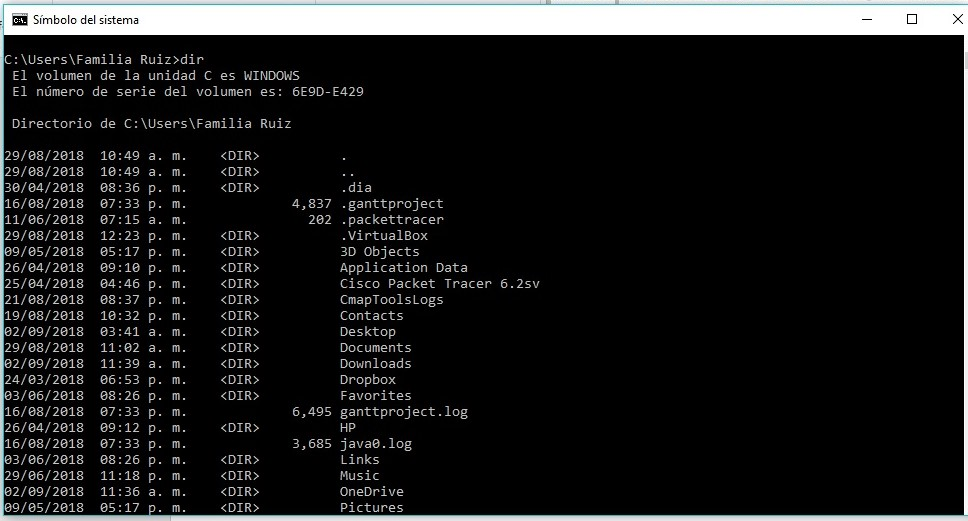
\includegraphics[scale=.6]{Imagenes/Windows/dir.jpg}	
			\item IPCONFIG: Muestra los valores de configuración de red de TCP/IP
			
				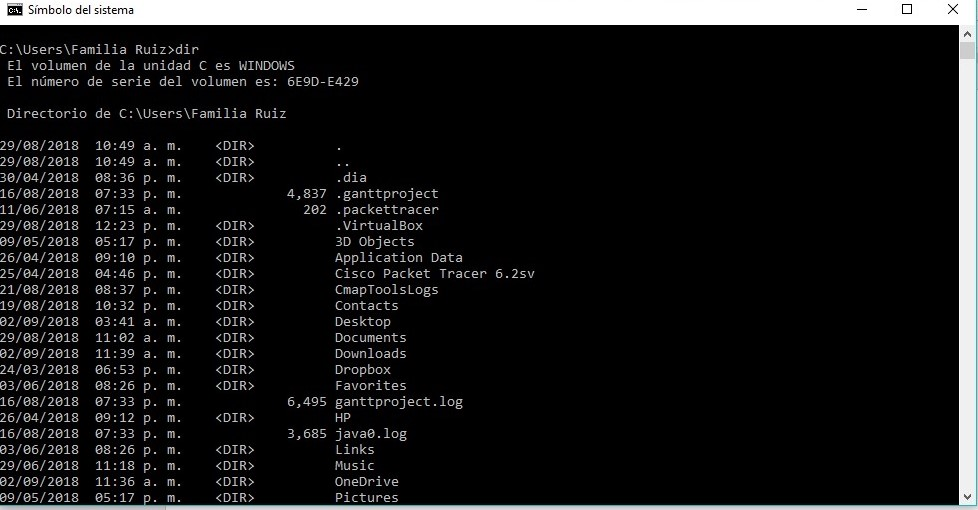
\includegraphics[scale=.6]{Imagenes/Windows/ipconfig.jpg}
			\newpage
			\item CLS: Borra la pantalla
			
				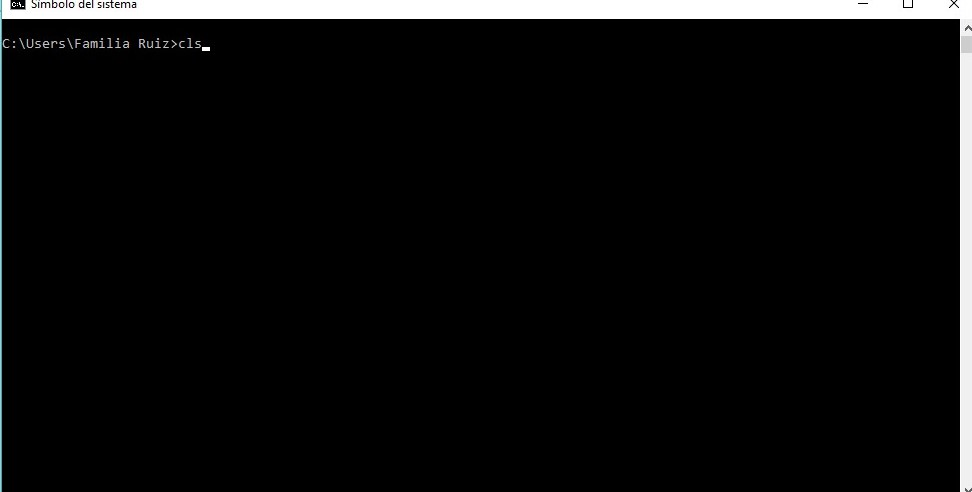
\includegraphics[scale=.6]{Imagenes/Windows/cls.jpg}	
			\item VER: Muestra la versión de Microsoft Windows
			
				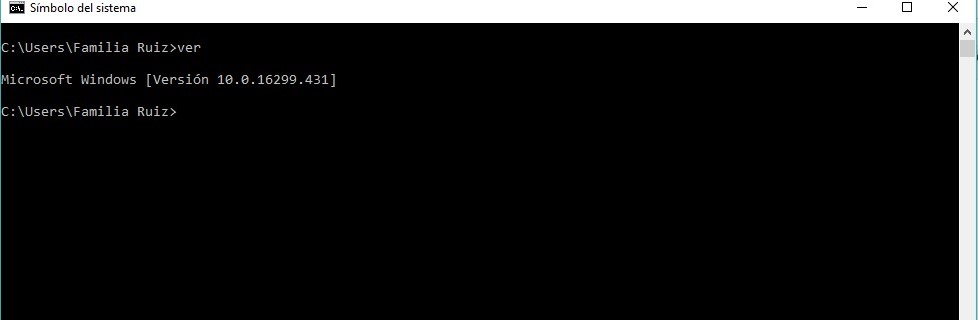
\includegraphics[scale=.6]{Imagenes/Windows/ver.jpg}	
			\item TREE: Muestra el listado de carpetas en Windows
			
				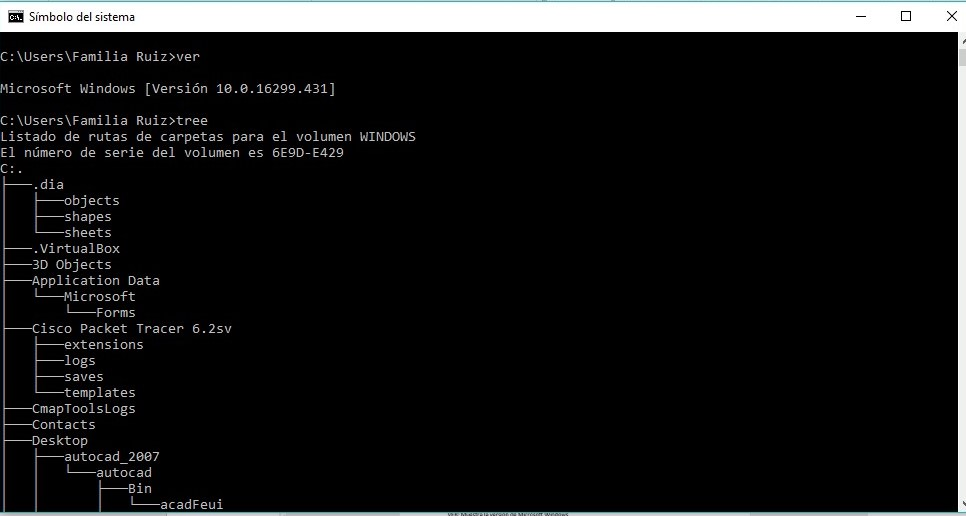
\includegraphics[scale=.5]{Imagenes/Windows/tree.jpg}\\	
			\item CD: Nos permite acceder a una carpeta o directorio de Windows
			
				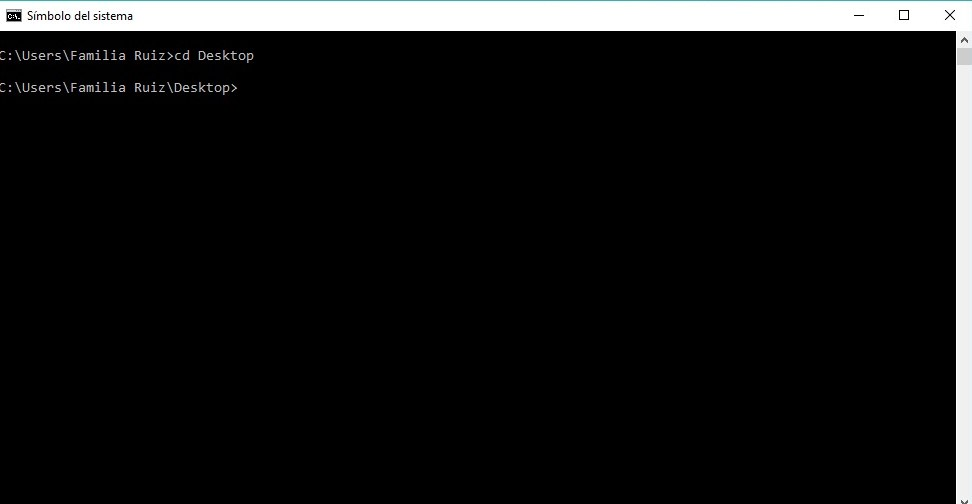
\includegraphics[scale=.6]{Imagenes/Windows/cd.jpg}	
			\item TYPE: Muestra el contenido de uno o más archivos de texto, es decir, la extensión
			
				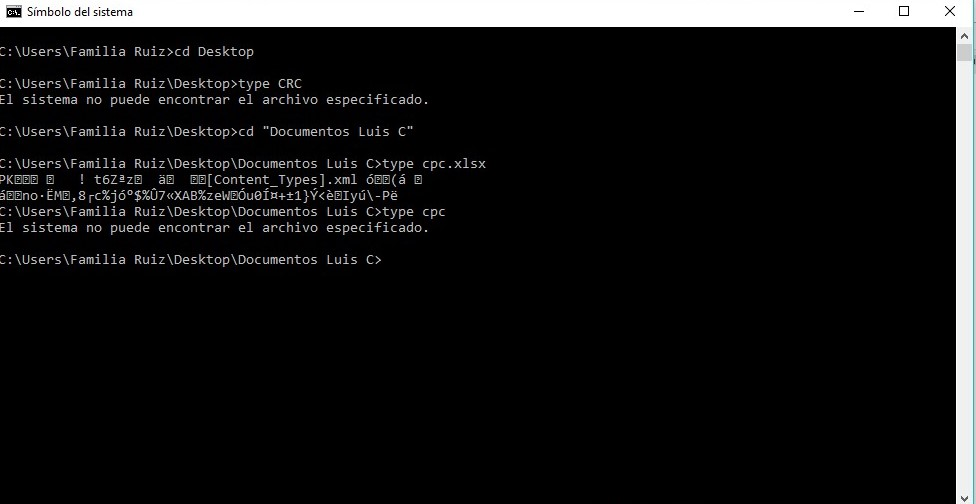
\includegraphics[scale=.6]{Imagenes/Windows/type.jpg}
			\newpage
			\item MKDIR:  Crea un directorio nuevo
			
				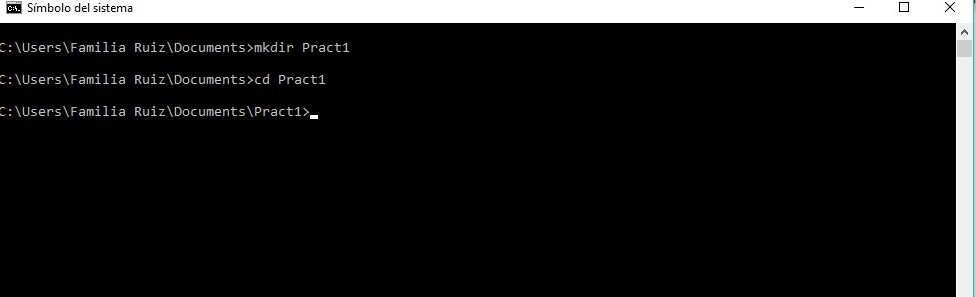
\includegraphics[scale=.6]{Imagenes/Windows/mkdir.jpg}	
				
			\item RMDIR: Borra un directorio existente
			
				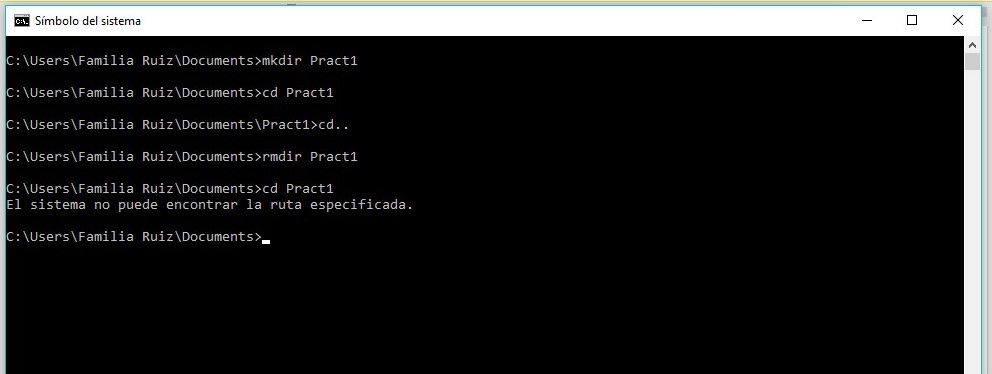
\includegraphics[scale=.6]{Imagenes/Windows/rmdir.jpg}	
			\item DEL: Elimina uno o varios archivos
			
				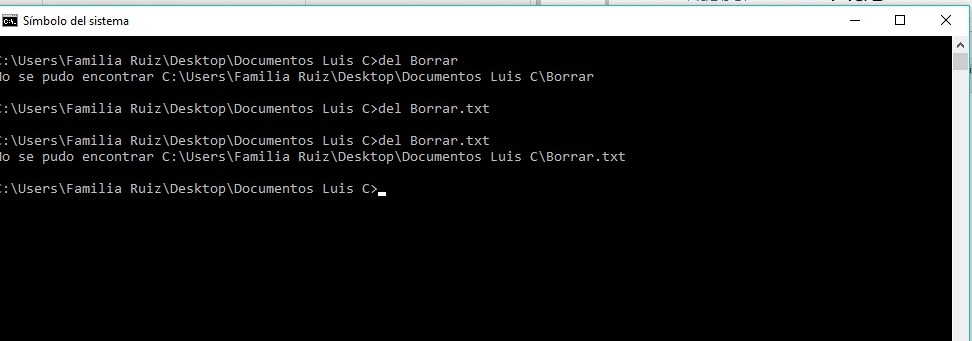
\includegraphics[scale=.6]{Imagenes/Windows/del.jpg}
			\newpage
			\item COPY: Copia un archivo
			
				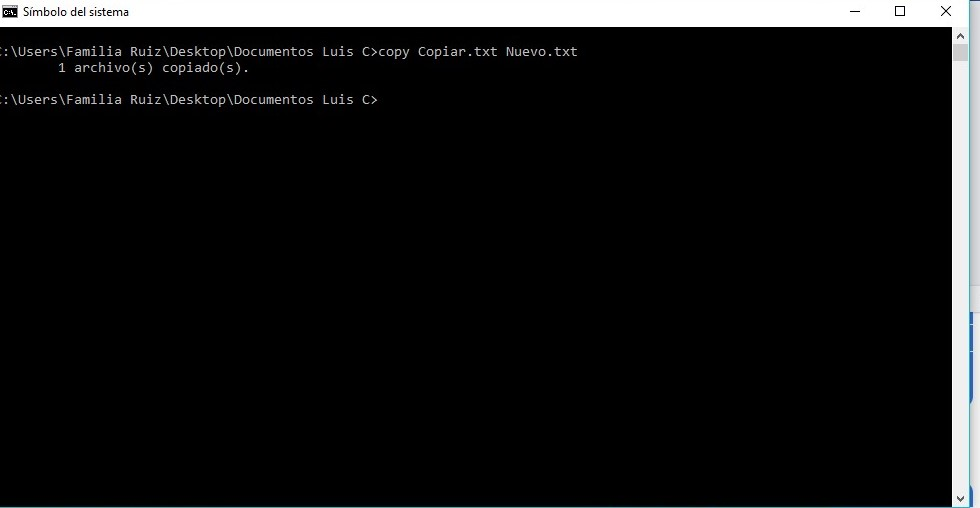
\includegraphics[scale=.6]{Imagenes/Windows/copy.jpg}	
			\item REN: Cambia el nombre de uno o más archivos
			
				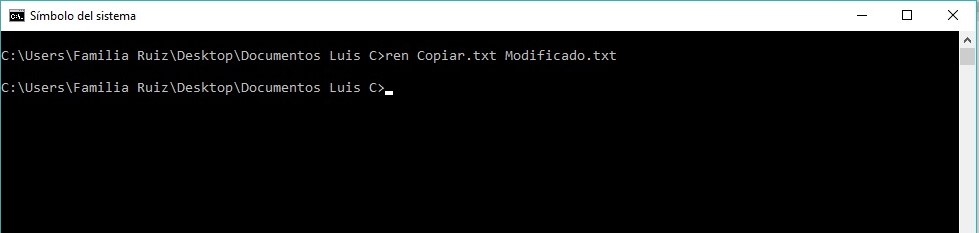
\includegraphics[scale=.6]{Imagenes/Windows/ren.jpg}	
			\item CHDIR: Muestra el nombre del directorio actual o cambia a otro directorio
			
				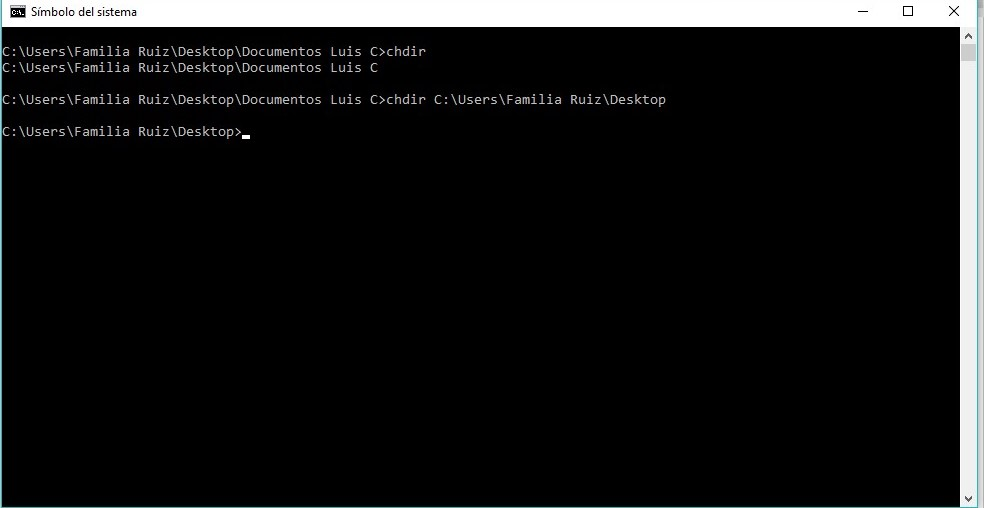
\includegraphics[scale=.6]{Imagenes/Windows/chdir.jpg}
				\\
			\item ECHO: Muestra mensajes o activa y desactiva al ECO
			
				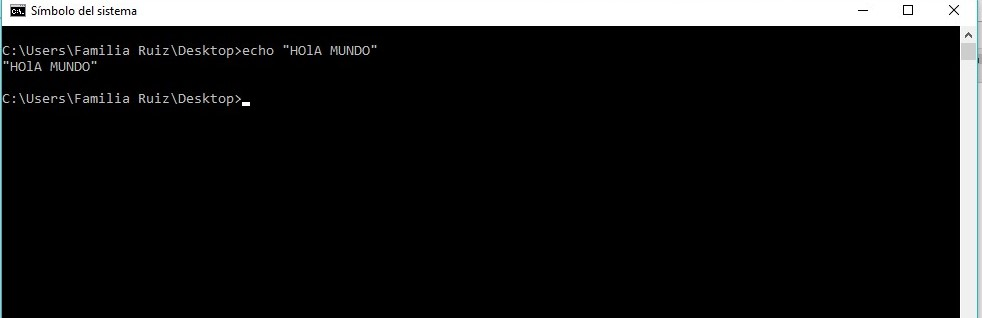
\includegraphics[scale=.6]{Imagenes/Windows/echo.jpg}
				
			\item FIND: Busca una cadena de texto en uno o más archivos
			
				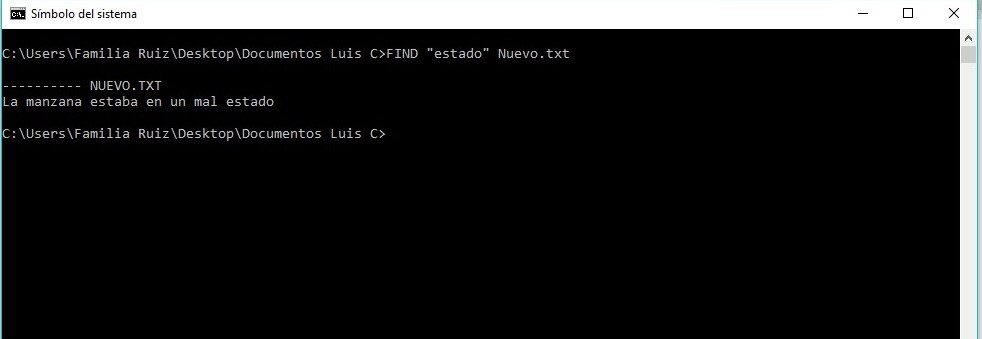
\includegraphics[scale=.6]{Imagenes/Windows/find.jpg}	
		\end{itemize}
\newpage	
\subsubsection{Compilación y ejecución}

\begin{itemize}
    \item \textbf{Busqueda directorio donde está instalado Dev C }
    
    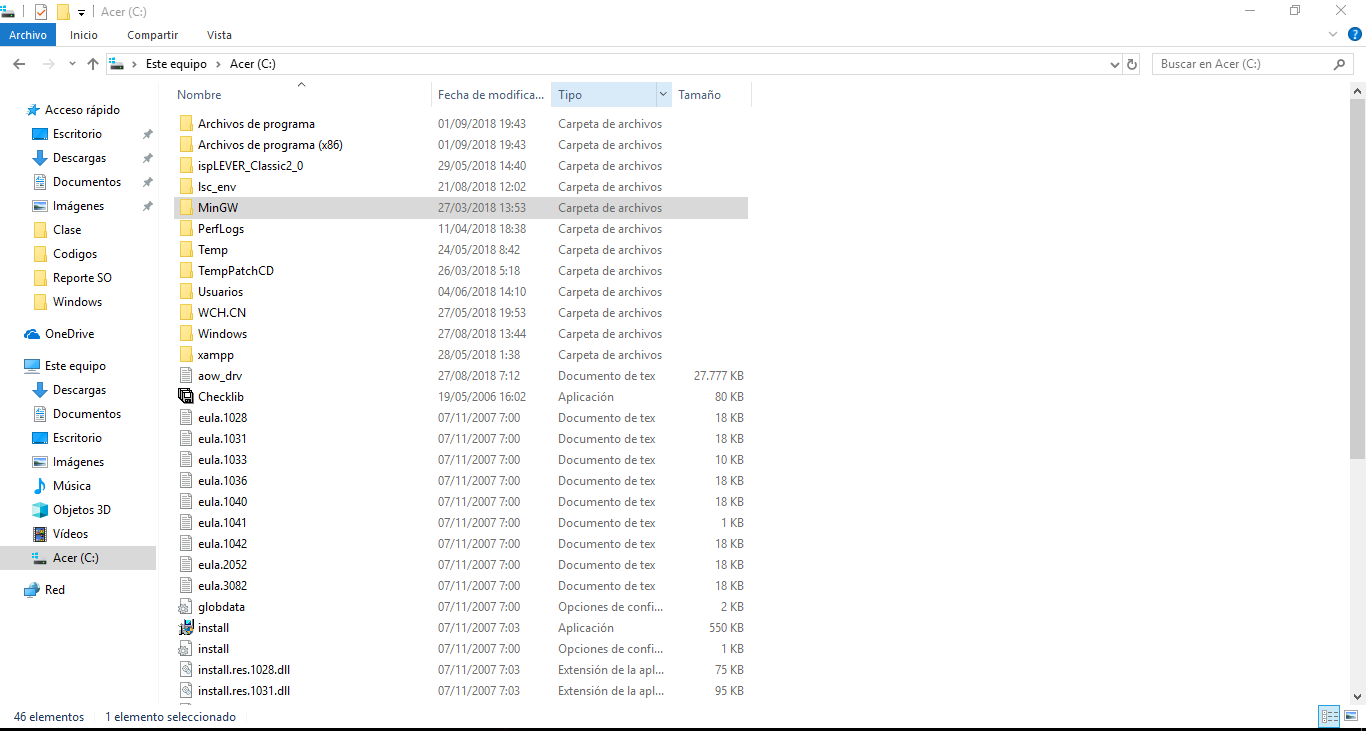
\includegraphics[scale=.5]{Imagenes/Windows/MinGw.PNG}
    
    \item \textbf{Cambio al directorio Bin, desde Consola}
 
     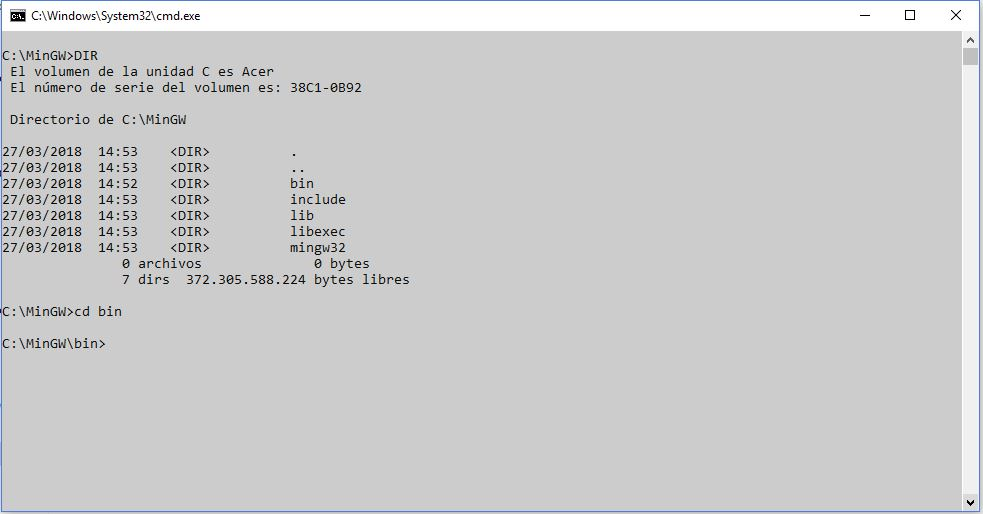
\includegraphics[scale=.6]{Imagenes/Windows/Bin.JPG}
     \newpage
    \item \textbf{Compilación en carpeta BIN}
    
    \begin{itemize}
                \item Hola Mundo
                
                   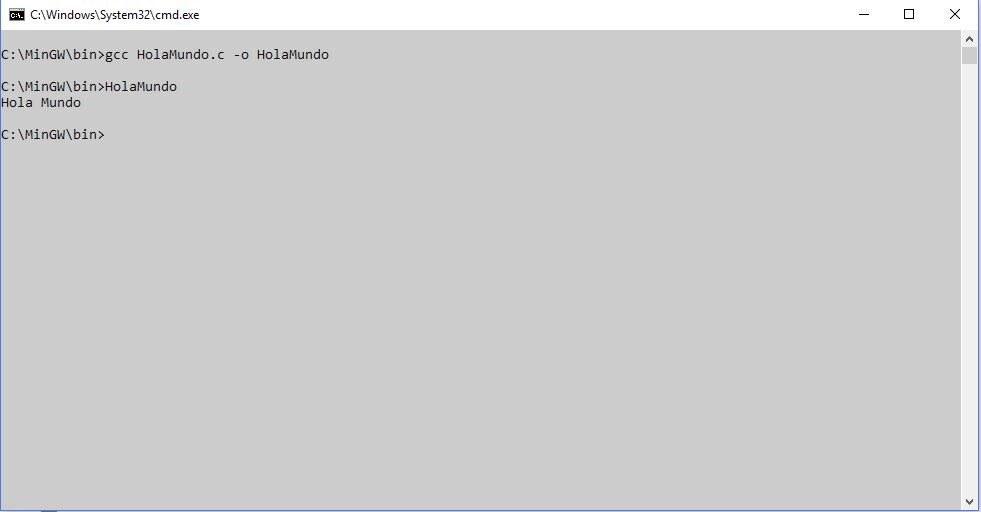
\includegraphics[scale=.6]{Imagenes/Windows/HolaMundo.JPG}
                   
                \item Balanceo de Paréntesis
                
                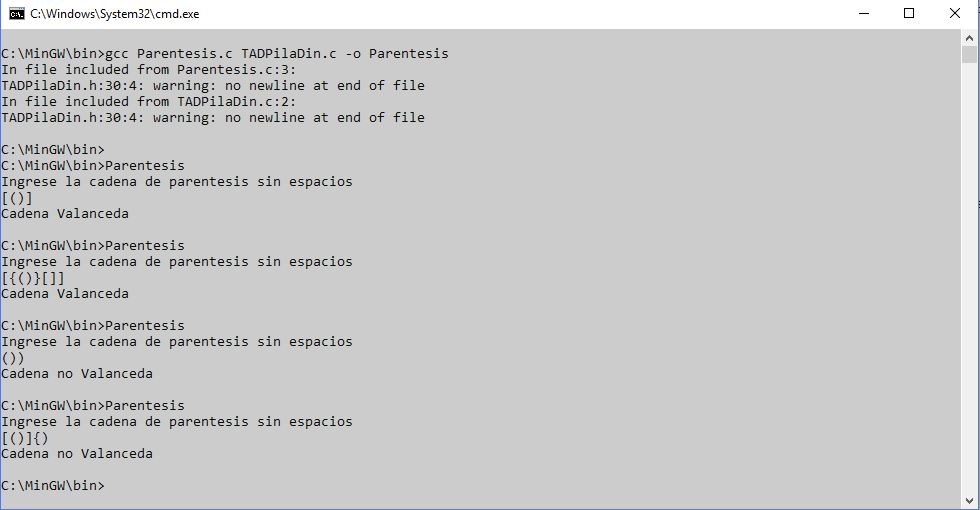
\includegraphics[scale=.6]{Imagenes/Windows/Parentesis.JPG}
                \newpage
                \item Salida de astesiscos
                
                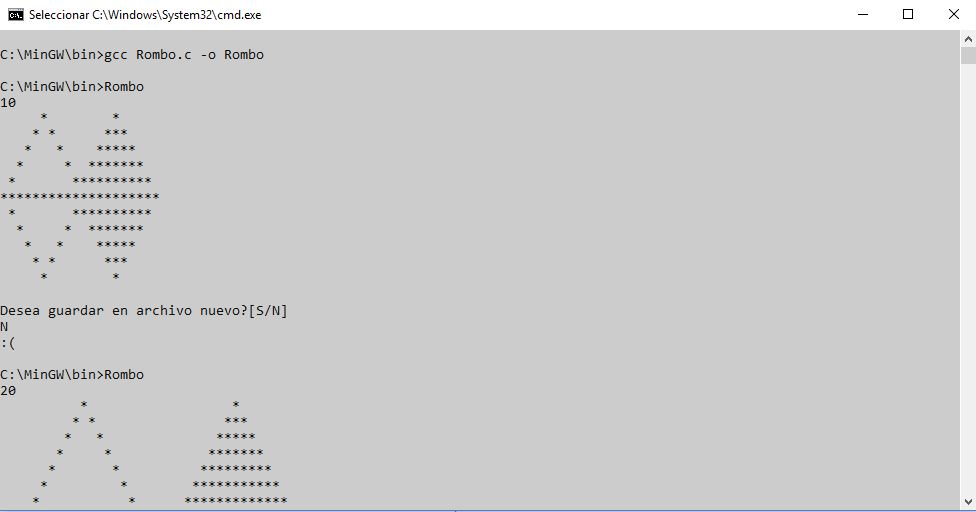
\includegraphics[scale=.6]{Imagenes/Windows/Asteriscos.JPG}

                \item Torres de Hanoi
                
                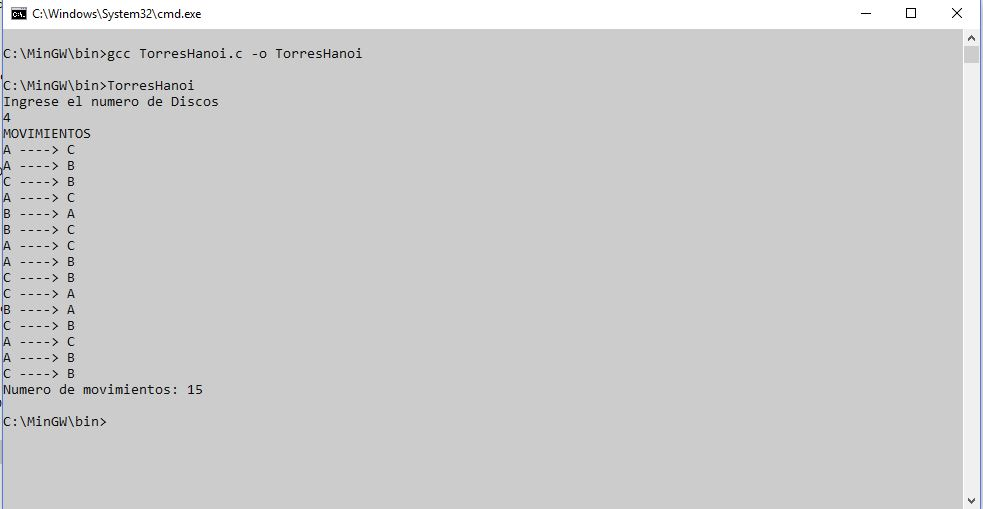
\includegraphics[scale=.6]{Imagenes/Windows/TorresHanoi.JPG}
                \newpage
                \item Expresiones Artiméticas\\
                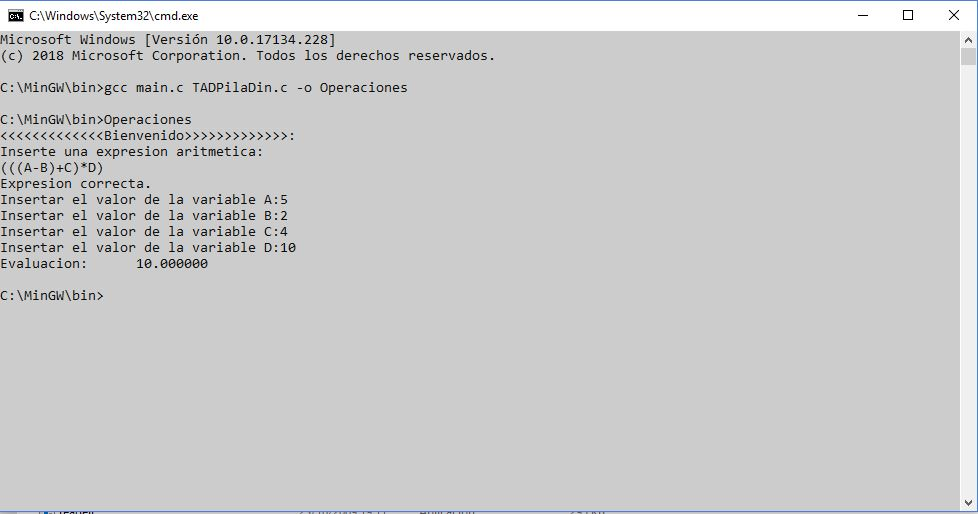
\includegraphics[scale=.6]{Imagenes/Windows/Operaciones.JPG}
                    
            \end{itemize}
    
\end{itemize}
\newpage    

\section{Código fuente.}
        \subsection{Hola Mundo} 
            \lstinputlisting{Codigos/HolaMundo.c}
        \subsection{Asteriscos}
            \lstinputlisting{Codigos/Rombo.c}
        \subsection{Balanceo de Paréntesis} 
                \subsubsection{Funciones de la Pila}
                    \lstinputlisting{Codigos/TADPilaDin.h}
                \subsubsection{Implementación de las funciones de la Pila}
                    \lstinputlisting{Codigos/TADPilaDin.c}
                \subsubsection{Implementación de la solución}
                    \lstinputlisting{Codigos/Parentesis.c}
        \subsection{Torres de Hanoi}
            \lstinputlisting{Codigos/TorresHanoi.c}
        \subsection{Expresiones Artiméticas}
            \lstinputlisting{Codigos/main.c}
\section{Observaciones.}

En cuanto a los comandos, pudimos observar que existen comandos muy similares o incluso iguales para ambos sistemas operativos. Algunos de ellos deben ser investigados más a fondo, ya que existen una gran variedad de éstos y no todos son tan sencillos de utilizar. De igual forma, debemos de saber con qué palabra o letras se ejecutan las funcionalidades deseadas para cada uno de los sistemas, ya que como vimos, algunos de éstos varían según el sistema. Es importante mencionar que debemos conocer la manera de compilar y ejecutar.

Por otro lado, la evaluación de una expresión aritmetica construyendo un árbol de expresión no fue posible implementarla por el hecho de que el árbol requeria ser un solo tipo de dato, sin embargo en la entrada encontrabamos una combinación de tipos de datos en la expresión, además que implicaba manejar una Pila, con direcciones de memoria, por lo que se opto por una evaluación con conversioón a postfijo por el hecho que implicaba el uso de un solo Tipo de Dato Abstracto.
\section{Análisis crítico.}

    Con lo visto en esta práctica, podemos ver que cada sistema operativo tiene sus funciones y cada uno trabaja a su forma. Teniendo en cuenta esto cada uno tiene sus ventajas y desventajas, las cuales nos permiten diferenciarlos y poderlos ocupar conforme a las tareas que queramos realizar.\\
    \begin{tabular}{||c|p{6.0cm}|p{6.0cm}||}
        \hline
        \hline & Windows & Linux\\ 
        \hline
        \hline Costes & Costes de licencia por usuario & Sin costes de licencia; los costes de asistencia dependen de las distribuciones\\
        \hline Uso estándar & Interfaz gráfica de usuario &	Líneas de comandos\\
        \hline Acceso remoto &Servidor de terminales;el cliente tiene que instalarse y configurarse & Solución integrada (terminal y shell)\\
        \hline Software y características & Soporta programas habituales; posibilidad de utilizar aplicaciones de Microsoft
            & No ofrece portabilidad para todos los programas; gran cantidad de aplicaciones disponibles\\
        \hline Soporte de hardware & El nuevo hardware está diseñado normalmente para los sistemas Windows
            & Por lo general, pueden utilizarse los controladores de hardware para las distribuciones de Linux más tarde\\
        \hline Seguridad & Elevado potencial de errores de usuario; interfaz integrada como posible punto de ataque 
            & Los usuarios habituales no tienen acceso a los ajustes básicos del sistema; las vulnerabilidades conocidas se solucionan rápidamente\\
        \hline Asistencia & Asistencia a largo plazo para todas las versiones &	La asistencia varía en función de la distribución y de la versión \\
        \hline Documentación & El sistema y sus aplicaciones están muy bien documentadas, algo que difiere de los componentes de la API y de los formatos de los datos &	Se conoce el código fuente completo del sistema, las API, las bibliotecas y las aplicaciones; la mayoría de manuales y de páginas informativas están en inglés\\
        \hline
        \hline
    \end{tabular}
    
\section{Conclusiones.}

Finalmente, por medio de la presente  práctica podemos concluir la importancia de conocer distintos sistemas operativos, ya que éstos tienen comandos, aplicaciones e interfaces distintas, así como el saber la manera de compilar y ejecutar un programa desde cada uno de éstos. Es importante saber diferenciar entre algunos sistemas operativos como apoyo a nuestro ambiente de trabajo, ya que cada sistema nos puede servir para realizar una tarea específica; pudimos notar que cada uno de ellos tiene ventajas y desventajas en su manera de trabajar.

Ahora bien. es importante destacar, que por la presente práctica, se recalca un objetivo de los desarrollores de software, que el algoritmo no este condicionado a la plataforma o sistema operativo en el que se ejecutara.







\end{document}



